\documentclass[]{elsarticle} %review=doublespace preprint=single 5p=2 column
%%% Begin My package additions %%%%%%%%%%%%%%%%%%%
\usepackage[hyphens]{url}

\usepackage{lineno} % add
\providecommand{\tightlist}{%
  \setlength{\itemsep}{0pt}\setlength{\parskip}{0pt}}

\usepackage{graphicx}
%%%%%%%%%%%%%%%% end my additions to header

\usepackage[T1]{fontenc}
\usepackage{lmodern}
\usepackage{amssymb,amsmath}
\usepackage{ifxetex,ifluatex}
\usepackage{fixltx2e} % provides \textsubscript
% use upquote if available, for straight quotes in verbatim environments
\IfFileExists{upquote.sty}{\usepackage{upquote}}{}
\ifnum 0\ifxetex 1\fi\ifluatex 1\fi=0 % if pdftex
  \usepackage[utf8]{inputenc}
\else % if luatex or xelatex
  \usepackage{fontspec}
  \ifxetex
    \usepackage{xltxtra,xunicode}
  \fi
  \defaultfontfeatures{Mapping=tex-text,Scale=MatchLowercase}
  \newcommand{\euro}{€}
\fi
% use microtype if available
\IfFileExists{microtype.sty}{\usepackage{microtype}}{}
\usepackage[left=3cm,right=3cm,top=3cm,bottom=3cm]{geometry}
\bibliographystyle{elsarticle-harv}
\usepackage{color}
\usepackage{fancyvrb}
\newcommand{\VerbBar}{|}
\newcommand{\VERB}{\Verb[commandchars=\\\{\}]}
\DefineVerbatimEnvironment{Highlighting}{Verbatim}{commandchars=\\\{\}}
% Add ',fontsize=\small' for more characters per line
\newenvironment{Shaded}{}{}
\newcommand{\AlertTok}[1]{\textcolor[rgb]{1.00,0.00,0.00}{#1}}
\newcommand{\AnnotationTok}[1]{\textcolor[rgb]{0.00,0.50,0.00}{#1}}
\newcommand{\AttributeTok}[1]{#1}
\newcommand{\BaseNTok}[1]{#1}
\newcommand{\BuiltInTok}[1]{#1}
\newcommand{\CharTok}[1]{\textcolor[rgb]{0.00,0.50,0.50}{#1}}
\newcommand{\CommentTok}[1]{\textcolor[rgb]{0.00,0.50,0.00}{#1}}
\newcommand{\CommentVarTok}[1]{\textcolor[rgb]{0.00,0.50,0.00}{#1}}
\newcommand{\ConstantTok}[1]{#1}
\newcommand{\ControlFlowTok}[1]{\textcolor[rgb]{0.00,0.00,1.00}{#1}}
\newcommand{\DataTypeTok}[1]{#1}
\newcommand{\DecValTok}[1]{#1}
\newcommand{\DocumentationTok}[1]{\textcolor[rgb]{0.00,0.50,0.00}{#1}}
\newcommand{\ErrorTok}[1]{\textcolor[rgb]{1.00,0.00,0.00}{\textbf{#1}}}
\newcommand{\ExtensionTok}[1]{#1}
\newcommand{\FloatTok}[1]{#1}
\newcommand{\FunctionTok}[1]{#1}
\newcommand{\ImportTok}[1]{#1}
\newcommand{\InformationTok}[1]{\textcolor[rgb]{0.00,0.50,0.00}{#1}}
\newcommand{\KeywordTok}[1]{\textcolor[rgb]{0.00,0.00,1.00}{#1}}
\newcommand{\NormalTok}[1]{#1}
\newcommand{\OperatorTok}[1]{#1}
\newcommand{\OtherTok}[1]{\textcolor[rgb]{1.00,0.25,0.00}{#1}}
\newcommand{\PreprocessorTok}[1]{\textcolor[rgb]{1.00,0.25,0.00}{#1}}
\newcommand{\RegionMarkerTok}[1]{#1}
\newcommand{\SpecialCharTok}[1]{\textcolor[rgb]{0.00,0.50,0.50}{#1}}
\newcommand{\SpecialStringTok}[1]{\textcolor[rgb]{0.00,0.50,0.50}{#1}}
\newcommand{\StringTok}[1]{\textcolor[rgb]{0.00,0.50,0.50}{#1}}
\newcommand{\VariableTok}[1]{#1}
\newcommand{\VerbatimStringTok}[1]{\textcolor[rgb]{0.00,0.50,0.50}{#1}}
\newcommand{\WarningTok}[1]{\textcolor[rgb]{0.00,0.50,0.00}{\textbf{#1}}}
\usepackage{longtable,booktabs,array}
\usepackage{calc} % for calculating minipage widths
% Correct order of tables after \paragraph or \subparagraph
\usepackage{etoolbox}
\makeatletter
\patchcmd\longtable{\par}{\if@noskipsec\mbox{}\fi\par}{}{}
\makeatother
% Allow footnotes in longtable head/foot
\IfFileExists{footnotehyper.sty}{\usepackage{footnotehyper}}{\usepackage{footnote}}
\makesavenoteenv{longtable}
\ifxetex
  \usepackage[setpagesize=false, % page size defined by xetex
              unicode=false, % unicode breaks when used with xetex
              xetex]{hyperref}
\else
  \usepackage[unicode=true]{hyperref}
\fi
\hypersetup{breaklinks=true,
            bookmarks=true,
            pdfauthor={},
            pdftitle={Livin' on the edge: Precision yield data shows evidence of ecosystem services from field boundaries},
            colorlinks=false,
            urlcolor=blue,
            linkcolor=magenta,
            pdfborder={0 0 0}}
\urlstyle{same}  % don't use monospace font for urls

\setcounter{secnumdepth}{5}
% Pandoc toggle for numbering sections (defaults to be off)

% Pandoc citation processing
\newlength{\cslhangindent}
\setlength{\cslhangindent}{1.5em}
\newlength{\csllabelwidth}
\setlength{\csllabelwidth}{3em}
% for Pandoc 2.8 to 2.10.1
\newenvironment{cslreferences}%
  {}%
  {\par}
% For Pandoc 2.11+
\newenvironment{CSLReferences}[2] % #1 hanging-ident, #2 entry spacing
 {% don't indent paragraphs
  \setlength{\parindent}{0pt}
  % turn on hanging indent if param 1 is 1
  \ifodd #1 \everypar{\setlength{\hangindent}{\cslhangindent}}\ignorespaces\fi
  % set entry spacing
  \ifnum #2 > 0
  \setlength{\parskip}{#2\baselineskip}
  \fi
 }%
 {}
\usepackage{calc}
\newcommand{\CSLBlock}[1]{#1\hfill\break}
\newcommand{\CSLLeftMargin}[1]{\parbox[t]{\csllabelwidth}{#1}}
\newcommand{\CSLRightInline}[1]{\parbox[t]{\linewidth - \csllabelwidth}{#1}\break}
\newcommand{\CSLIndent}[1]{\hspace{\cslhangindent}#1}

% Pandoc header
\makeatletter \def\ps@pprintTitle{  \let\@oddhead\@empty  \let\@evenhead\@empty  \def\@oddfoot{\centerline{\thepage}} \let\@evenfoot\@oddfoot} \makeatother \usepackage{float} \floatplacement{figure}{H} \newcommand{\beginsupplement}{\setcounter{table}{0} \renewcommand{\thetable}{S\arabic{table}} \setcounter{figure}{0} \renewcommand{\thefigure}{S\arabic{figure}}} 
\usepackage{booktabs}
\usepackage{longtable}
\usepackage{array}
\usepackage{multirow}
\usepackage{wrapfig}
\usepackage{float}
\usepackage{colortbl}
\usepackage{pdflscape}
\usepackage{tabu}
\usepackage{threeparttable}
\usepackage{threeparttablex}
\usepackage[normalem]{ulem}
\usepackage{makecell}
\usepackage{xcolor}

\begin{document}

\hypertarget{figures}{%
\section*{Figures and Tables}\label{figures}}

\begin{figure}
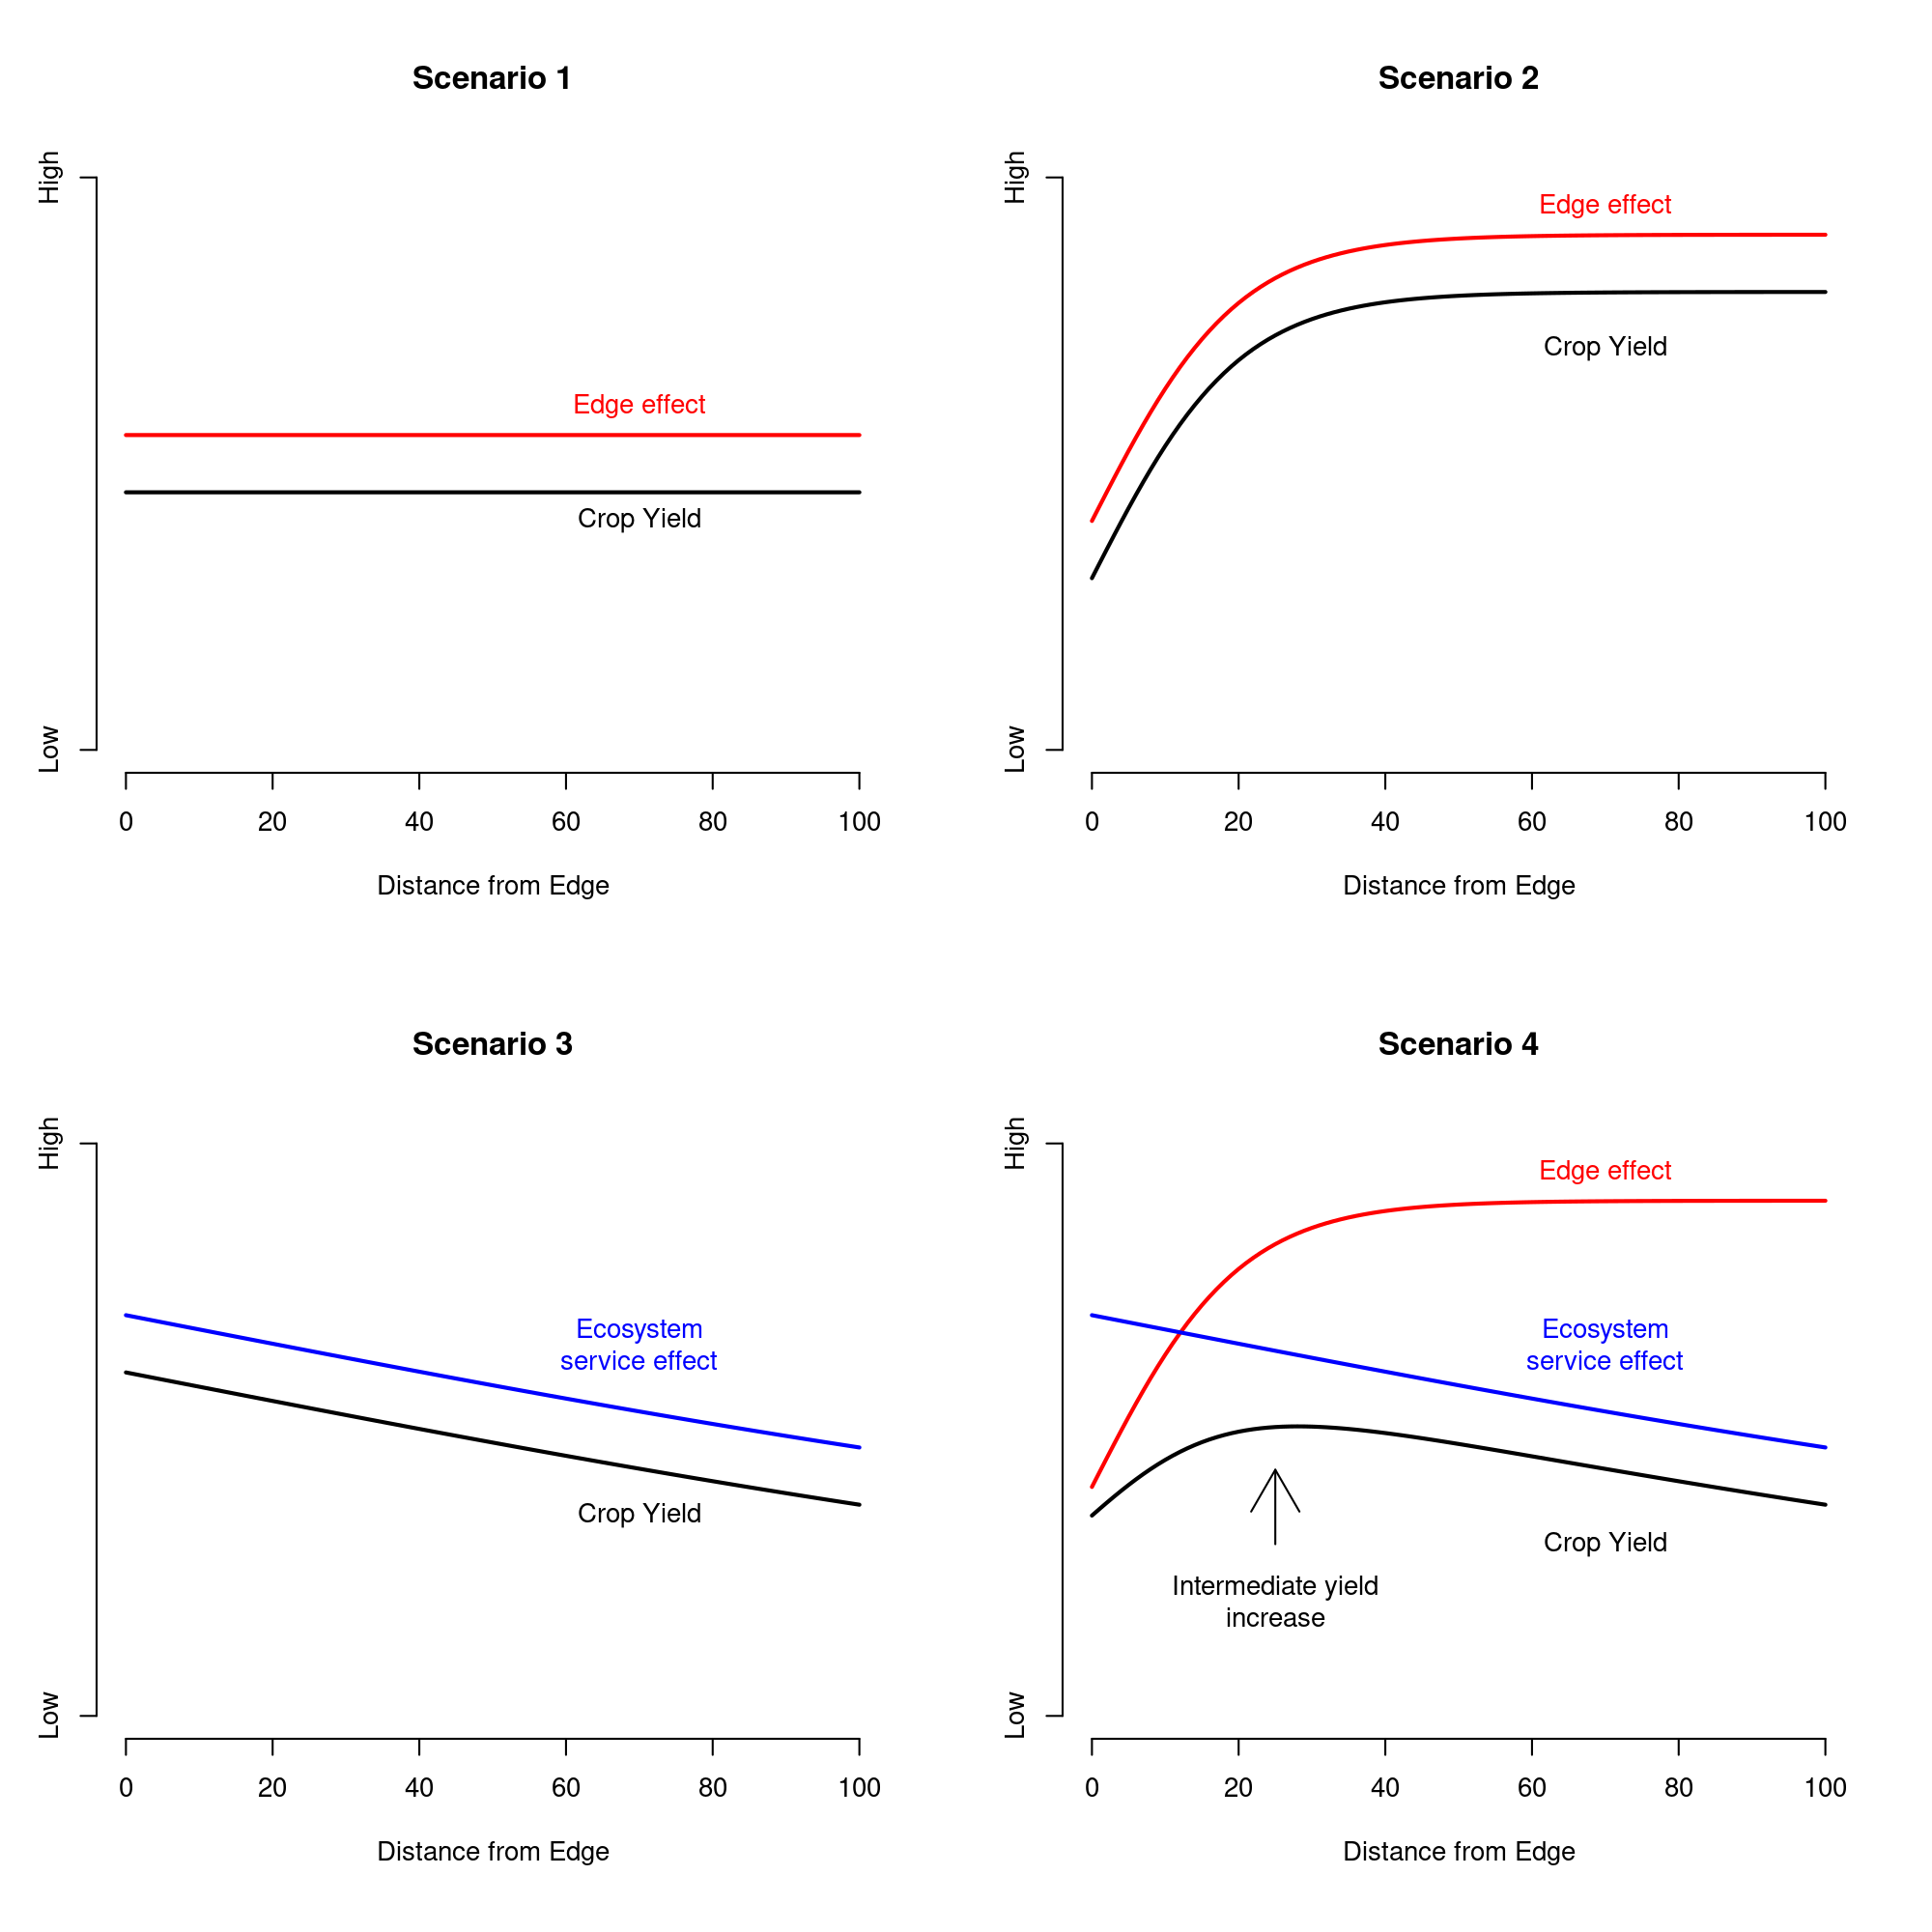
\includegraphics[width=1\linewidth]{hypotheses} \caption{Potential yield patterns, depending on ecosystem service effects with distance. Scenario 1: no effect of boundary. Scenario 2: negative edge effect on yield. Scenario 3: positive ecosystem service effect on yield. Scenario 4: edge effects are shown in red, ecosystem service effect shown blue, leading to an intermediate peak in yield.}
\end{figure}

\newpage

\begin{figure}
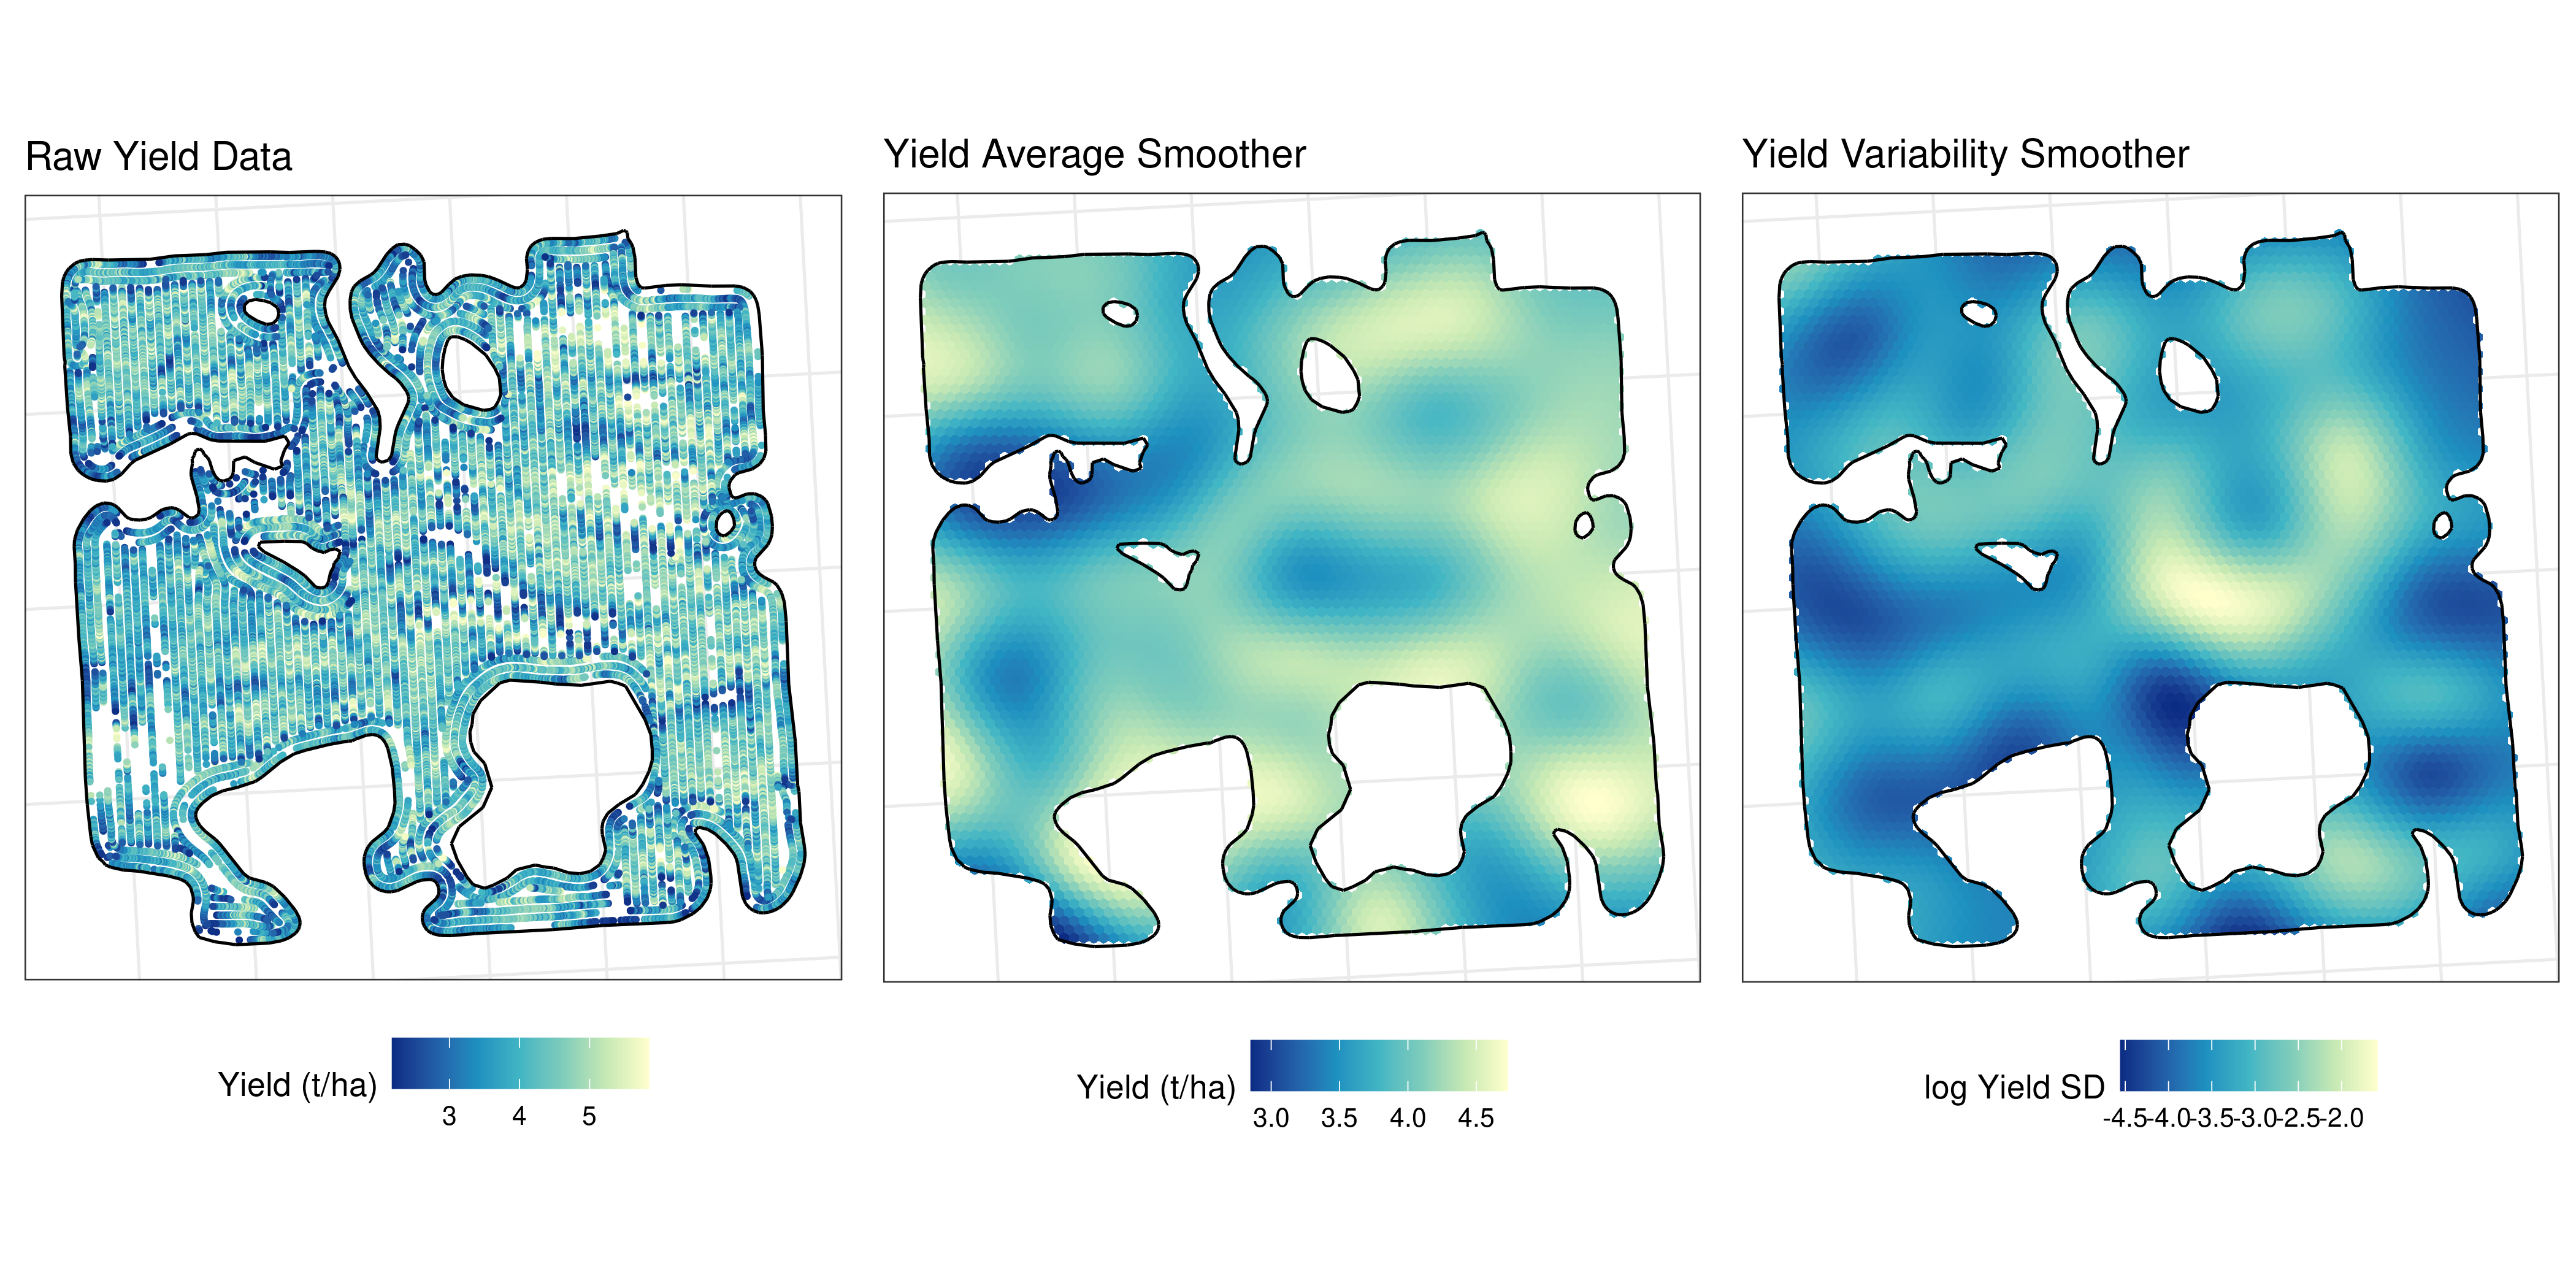
\includegraphics[width=1\linewidth]{spatialSmooths} \caption{Raw data and spatial smoothers from a single field. Yield averages (means) and variability (log SD) were modeled separately, and both show large spatial dependence within the field. Field dimensions are approximately 800 x 800 m; coordinates are hidden to protect the grower's data privacy.}
\end{figure}

\newpage

\begin{figure}
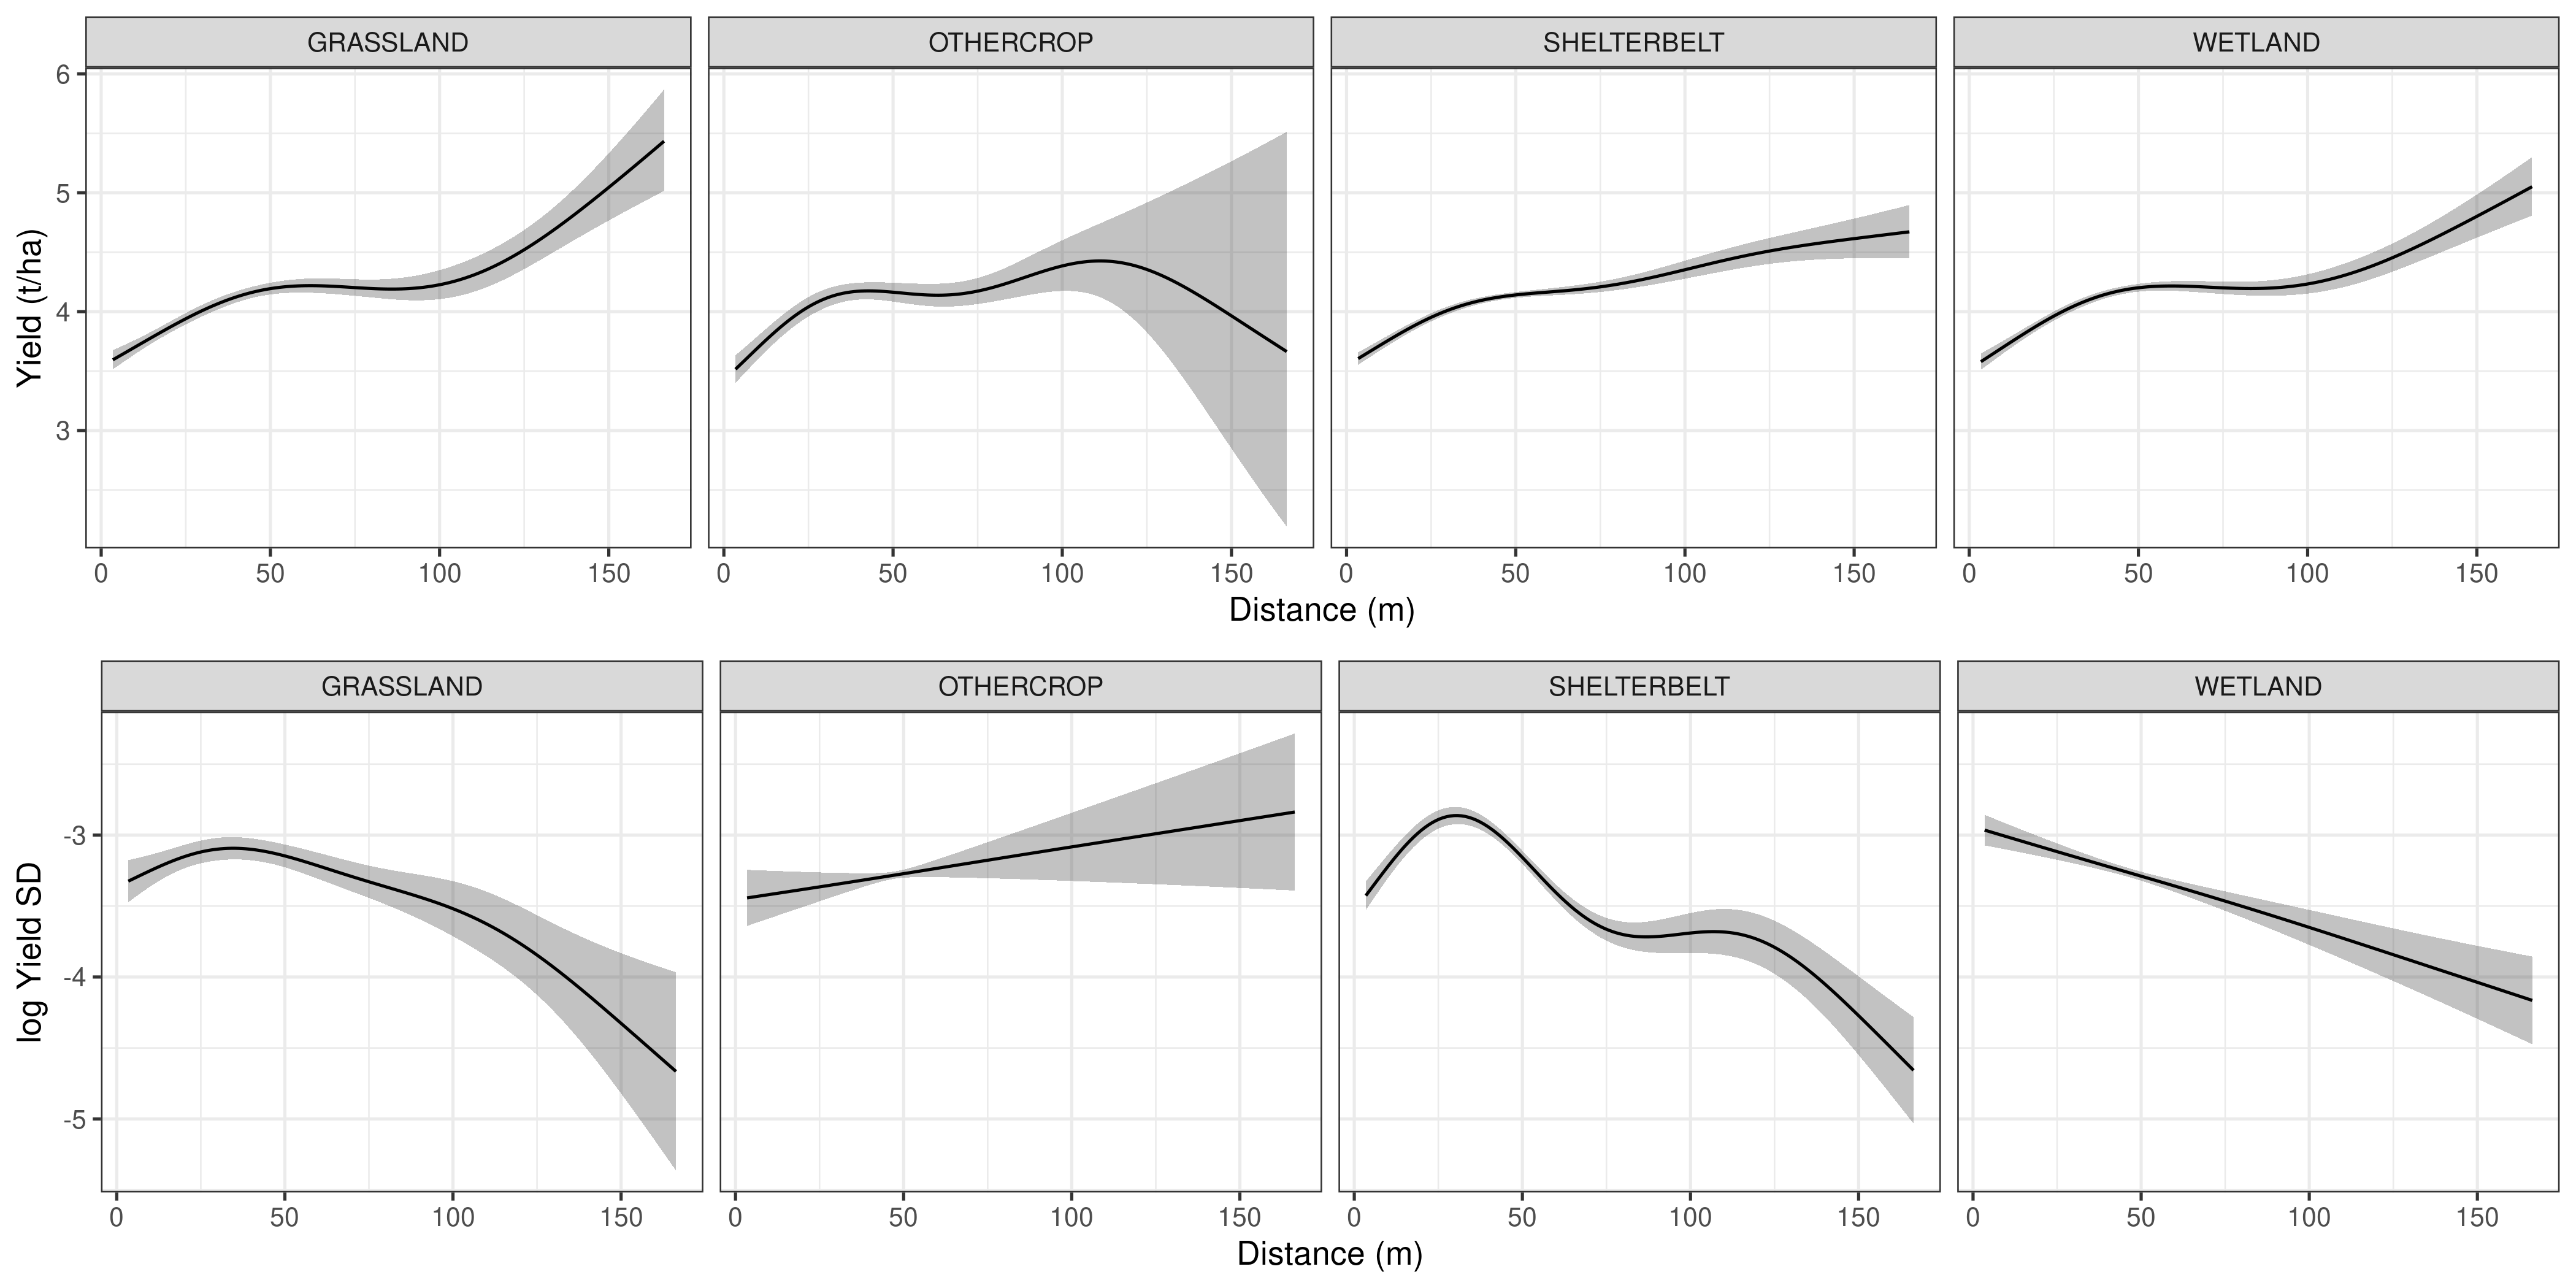
\includegraphics[width=1\linewidth]{distSmooths} \caption{Distance smoothers from a single field, showing a positive saturating effect of distance on average yield (first row), while the variability smoothers show a general decrease in yield SD (second row).}
\end{figure}

\newpage

\begin{figure}
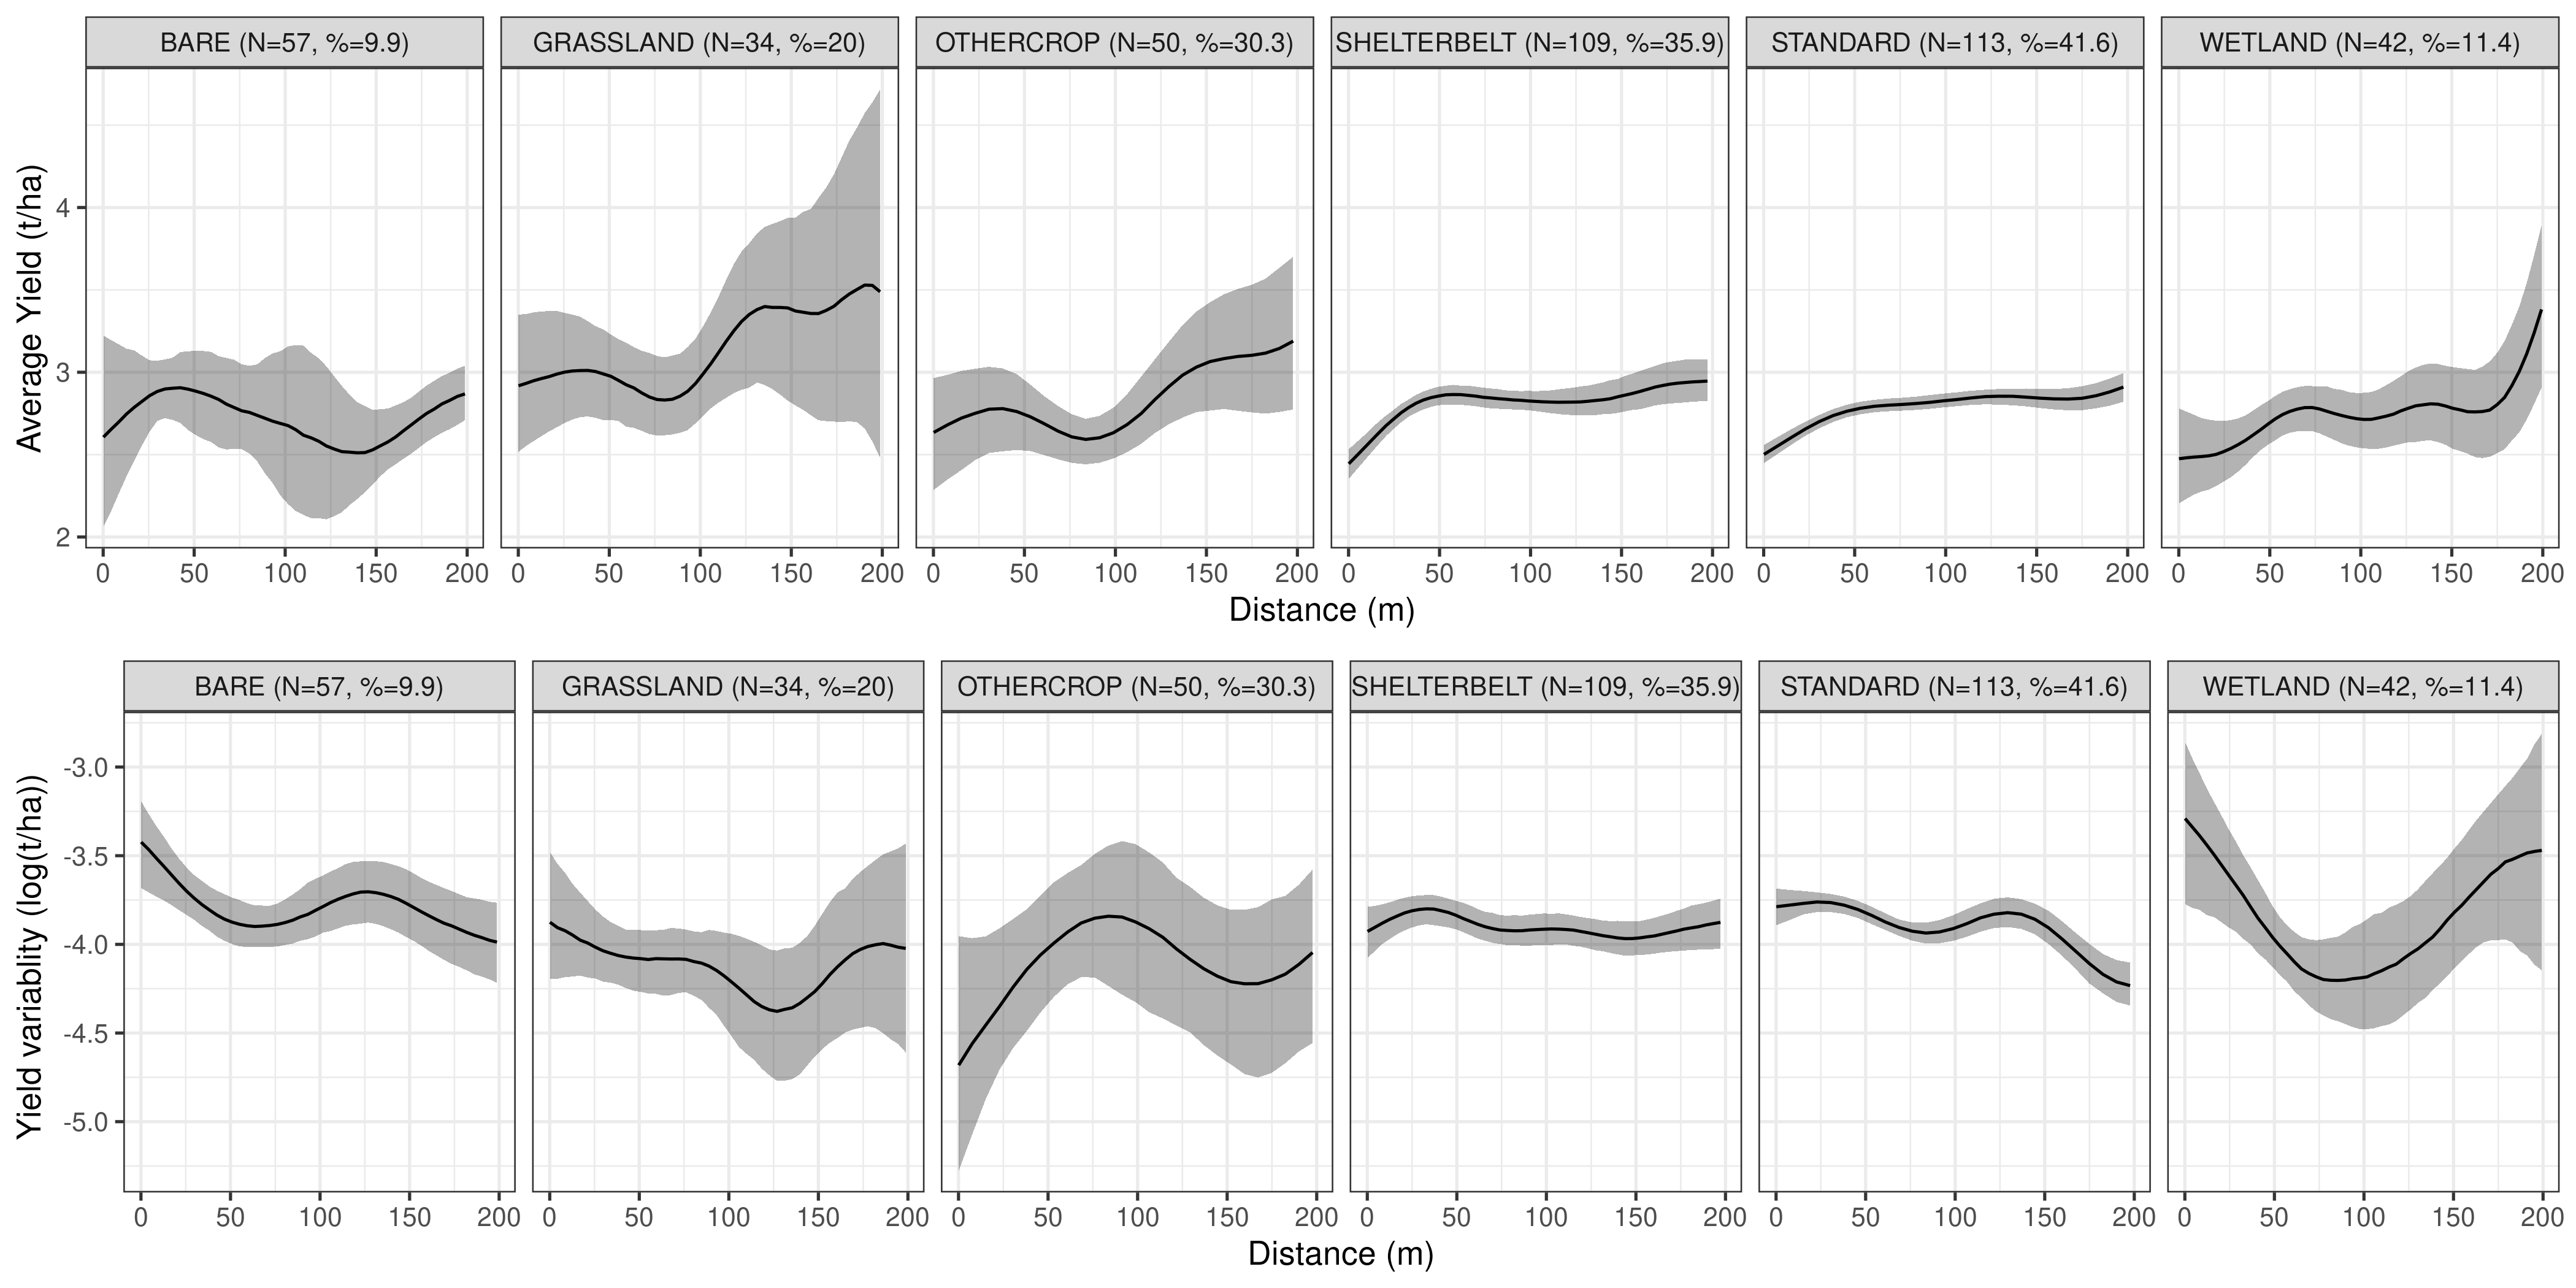
\includegraphics[width=1\linewidth]{ModelSummary3a_canola} \caption{Field boundary effect on canola yield, accounting for the effect of spatial variation. Upper panel represents mean yield, while the lower panel represents yield variation. N refers to number of fields containing this boundary type, and \% refers to the average percentage of field boundary accounted for by this boundary type.}
\end{figure}

\newpage

\begin{figure}
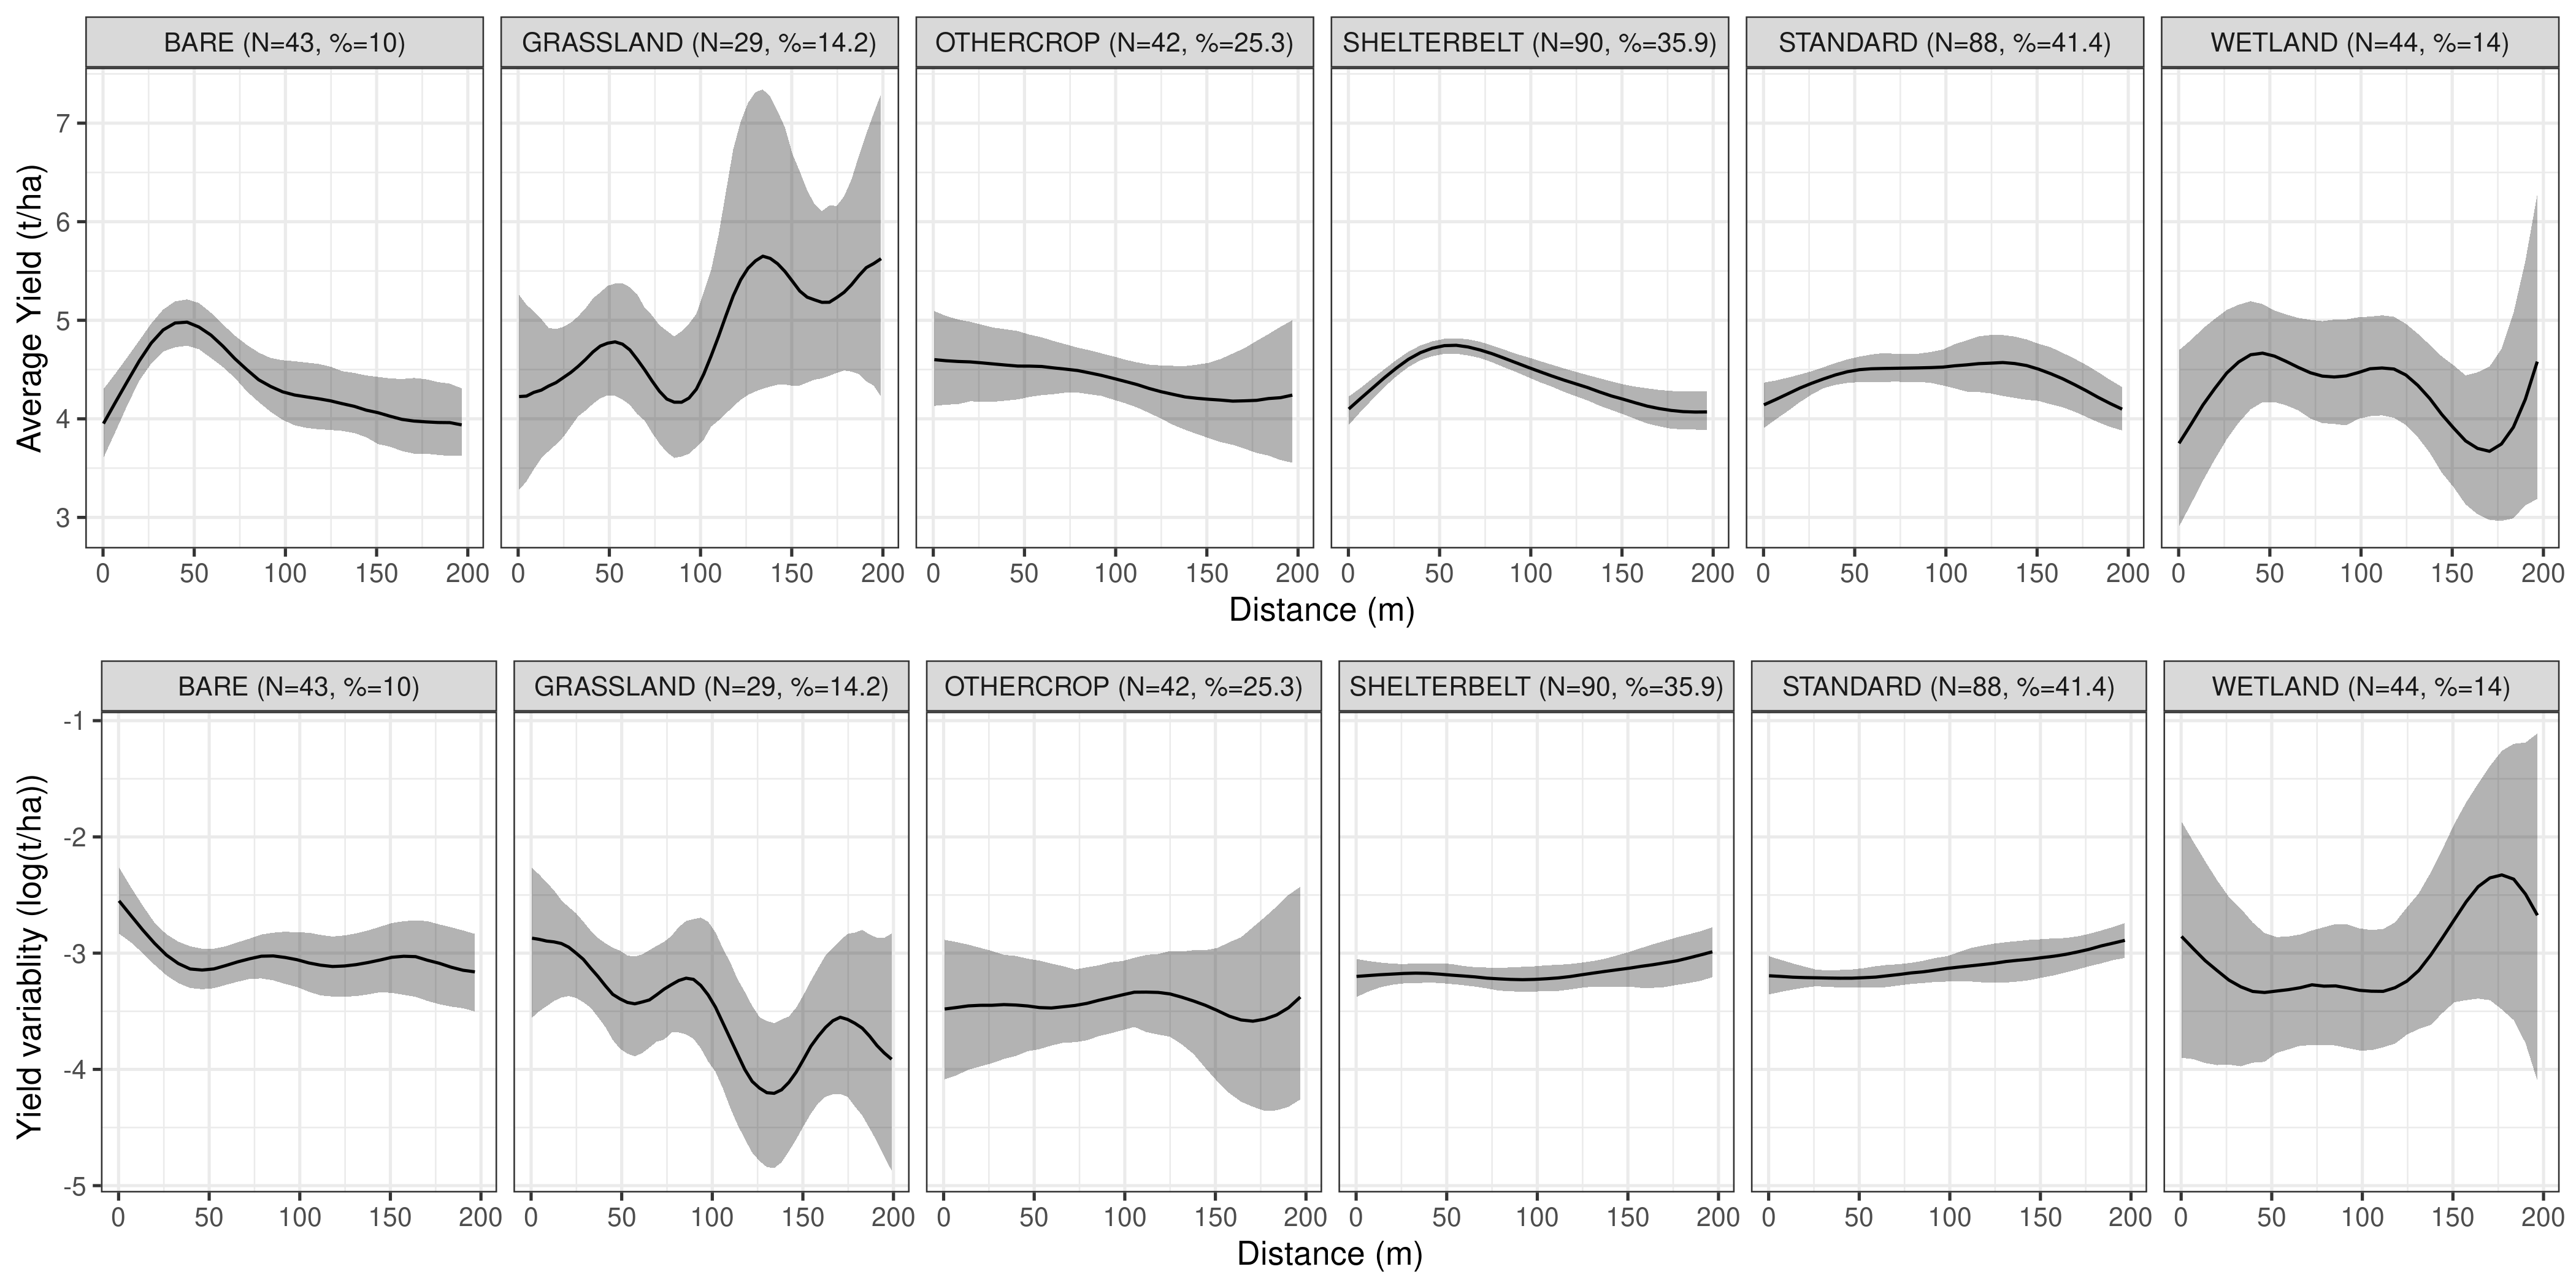
\includegraphics[width=1\linewidth]{ModelSummary3a_wheat} \caption{Field boundary effect on wheat yield, accounting for the effect of spatial variation. Upper panel represents mean yield, while the lower panel represents yield variation. N refers to number of fields containing this boundary type, and \% refers to the average percentage of field boundary accounted for by this boundary type.}
\end{figure}

\newpage

\begin{figure}
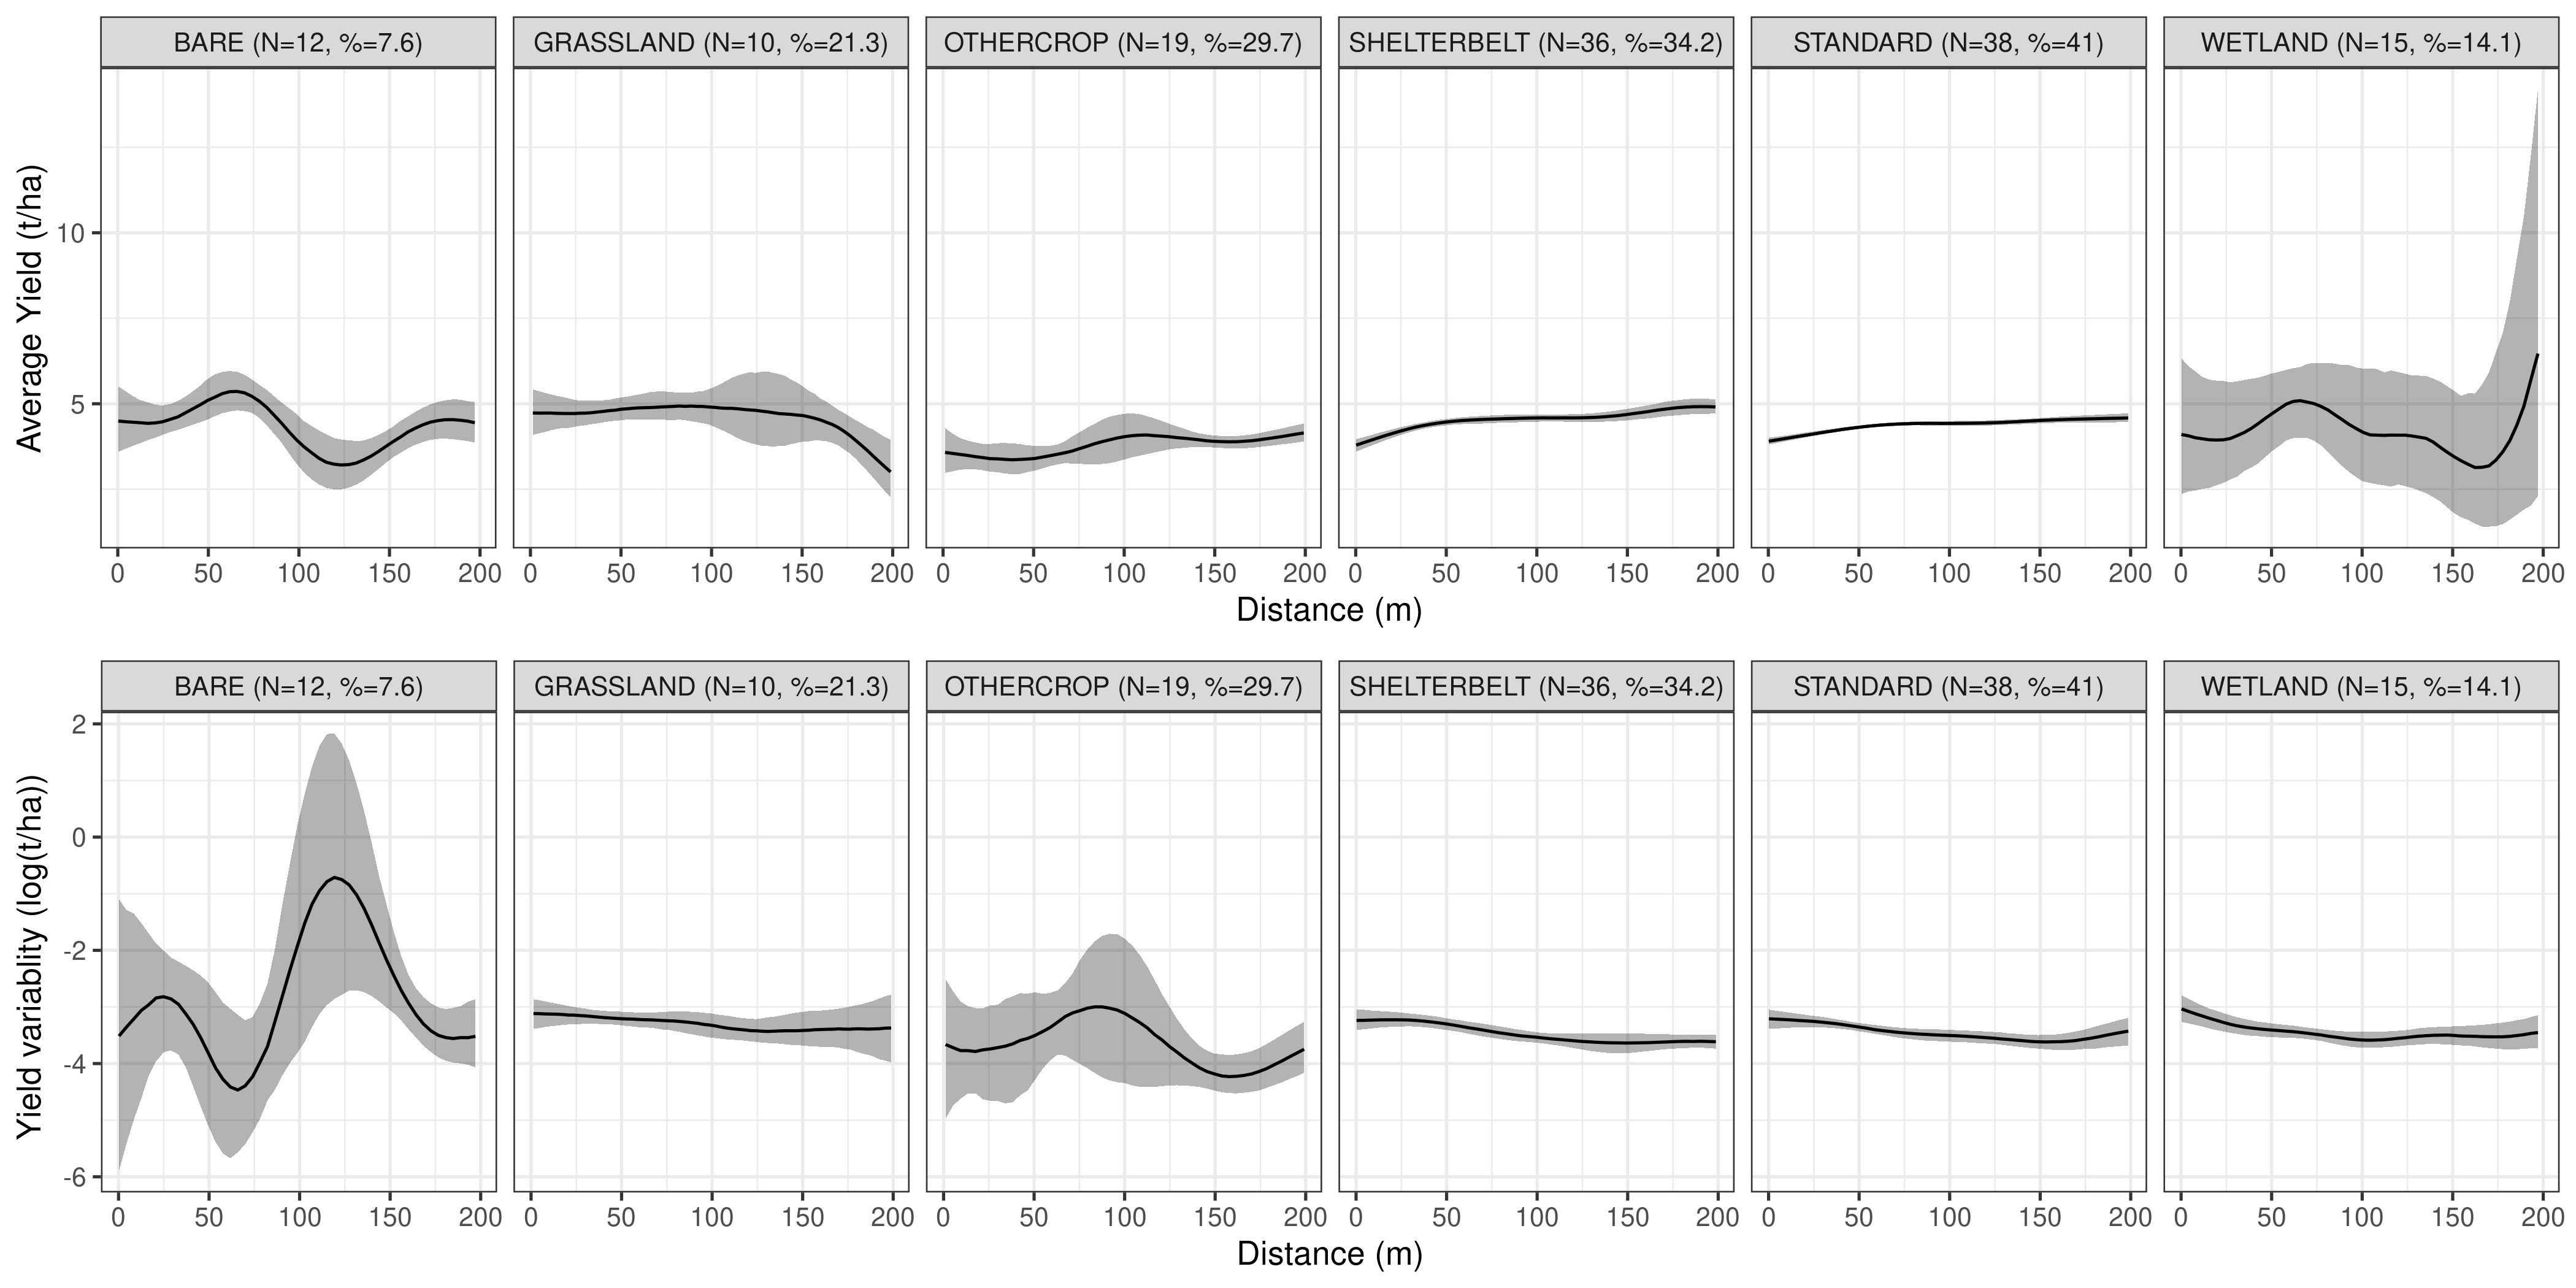
\includegraphics[width=1\linewidth]{ModelSummary3a_peas} \caption{Field boundary effect on pea yield, accounting for the effect of spatial variation. Upper panel represents mean yield, while the lower panel represents yield variation. N refers to number of fields containing this boundary type, and \% refers to the average percentage of field boundary accounted for by this boundary type.}
\end{figure}

\newpage

\begin{table}

\caption{Mean $\chi^2$, p-values, and proportion of smoother p-values less than 0.05 (after Bonneferoni correction) for mean and variability smoothers across all models.}
\centering
\begin{tabular}[H]{l|r|r|r|r|r|r}
\hline
\multicolumn{1}{c|}{} & \multicolumn{3}{c|}{Mean Yield} & \multicolumn{3}{c}{Yield Variability} \\
\cline{2-4} \cline{5-7}
Smoother Type & $\chi^2$-value & p-value & Prop. <0.05 & $\chi^2$-value & p-value & Prop. <0.05\\
\hline
Bare & 154.7 & 0.036 & 0.877 & 121.4 & 0.054 & 0.860\\
\hline
Grassland & 303.1 & 0.079 & 0.794 & 93.2 & 0.061 & 0.794\\
\hline
Other Crop & 174.9 & 0.063 & 0.860 & 104.5 & 0.044 & 0.840\\
\hline
Shelterbelt & 328.1 & 0.014 & 0.936 & 137.6 & 0.058 & 0.817\\
\hline
Standard & 281.9 & 0.021 & 0.938 & 159.6 & 0.057 & 0.832\\
\hline
Wetland & 148.9 & 0.045 & 0.833 & 106.7 & 0.013 & 0.857\\
\hline
Spatial Smoother & 17357.5 & 0.000 & 1.000 & 4739.1 & 0.000 & 1.000\\
\hline
\end{tabular}
\end{table}

\end{document}
